\section{Runtime view}
\label{sec:runtime-view}

In this section we will describe the dynamic behaviour of the system.
In particular, it will be shown how the software and logical components defined in \autoref{sec:component-view} interact one with another, using \emph{sequence diagrams} for the more meaningful functionalities of the system.
We decided not to represent the database in the sequence diagram, because the interaction witht the database is totally abstracted by the entities via the Java Persistence API.

Also, \emph{runtime unit diagrams} will be shown in some use cases of the software: these diagrams show the instances of the components running in the tiers when the users interact with the system.

\begin{figure}[h]
    \centering
    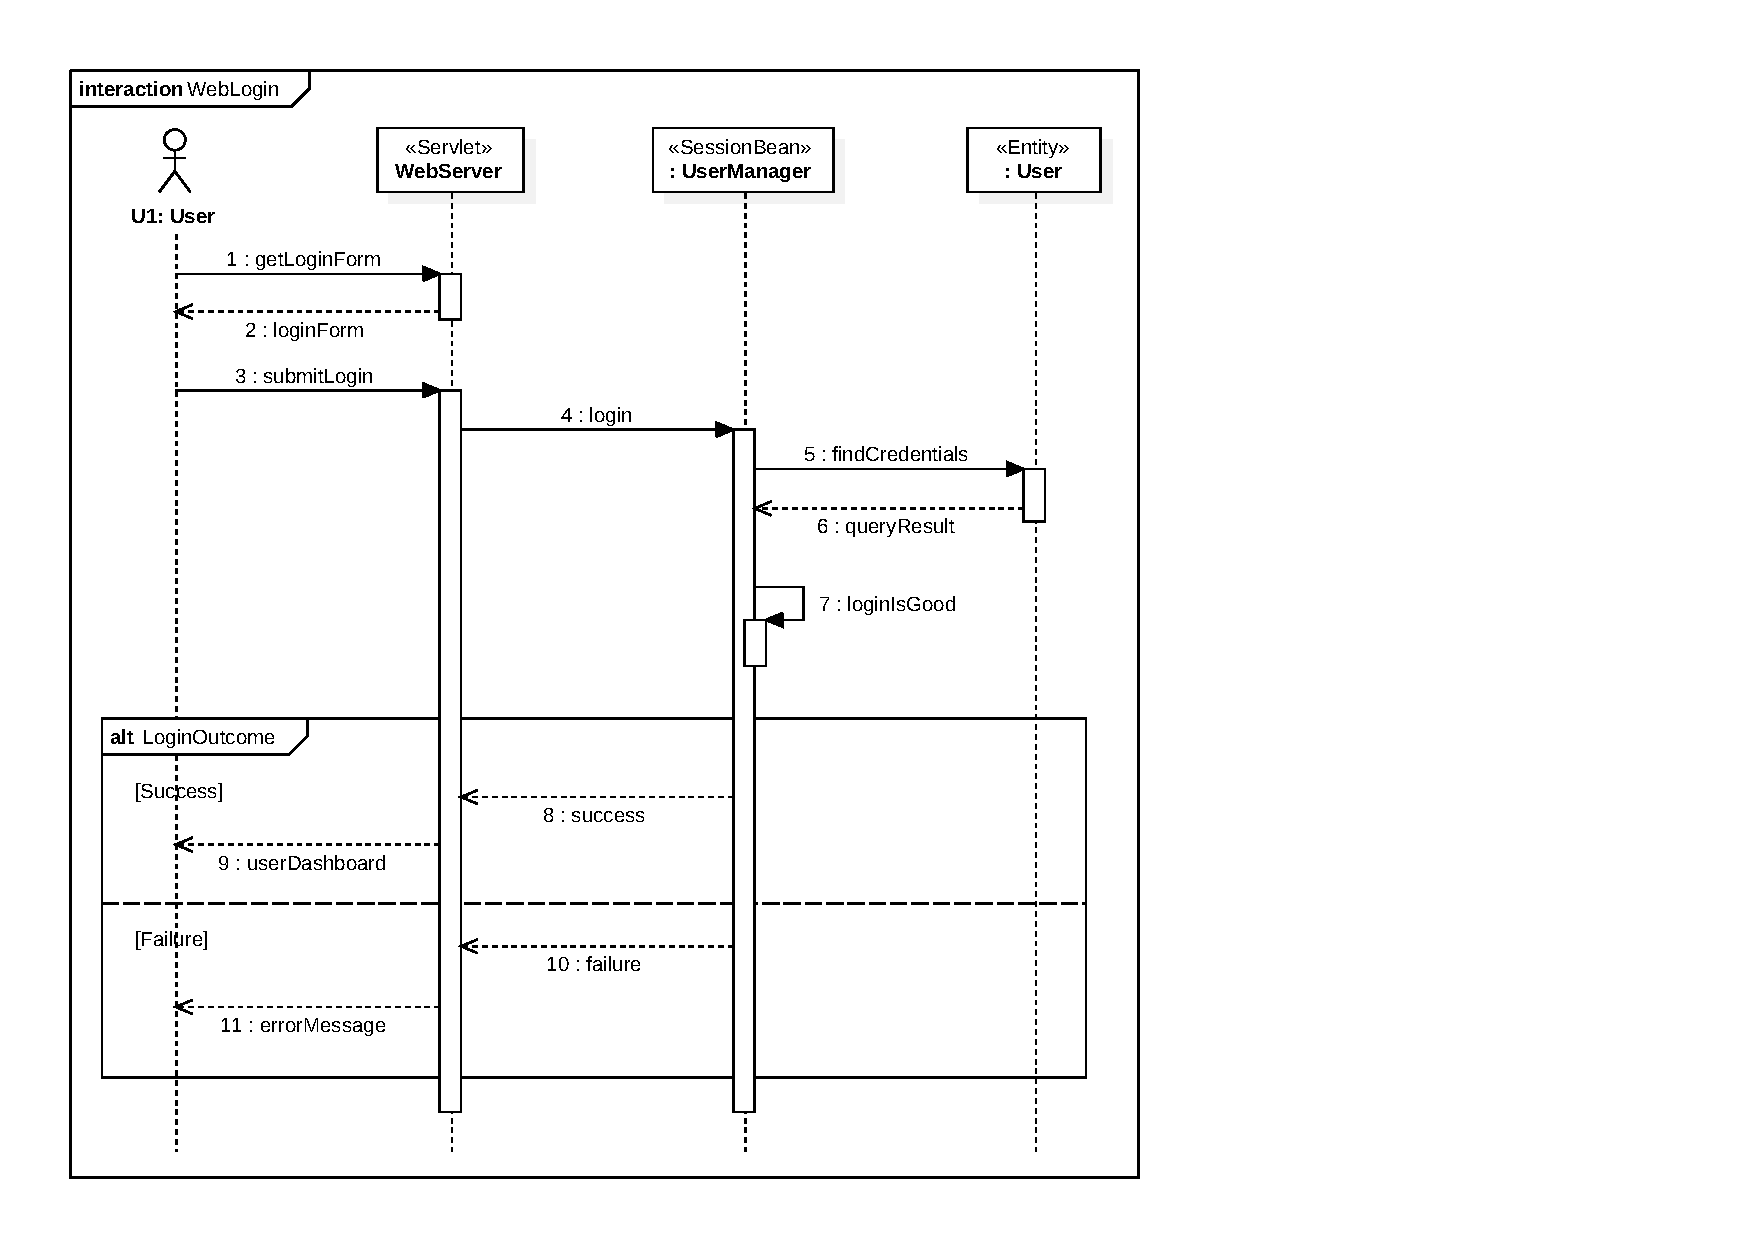
\includegraphics[width=\textwidth]{diagrams/sequence_weblogin}
    \caption{Sequence diagram of the login with the web interface.}
    \label{fig:sequence-weblogin}
\end{figure}

\begin{figure}[h]
    \centering
    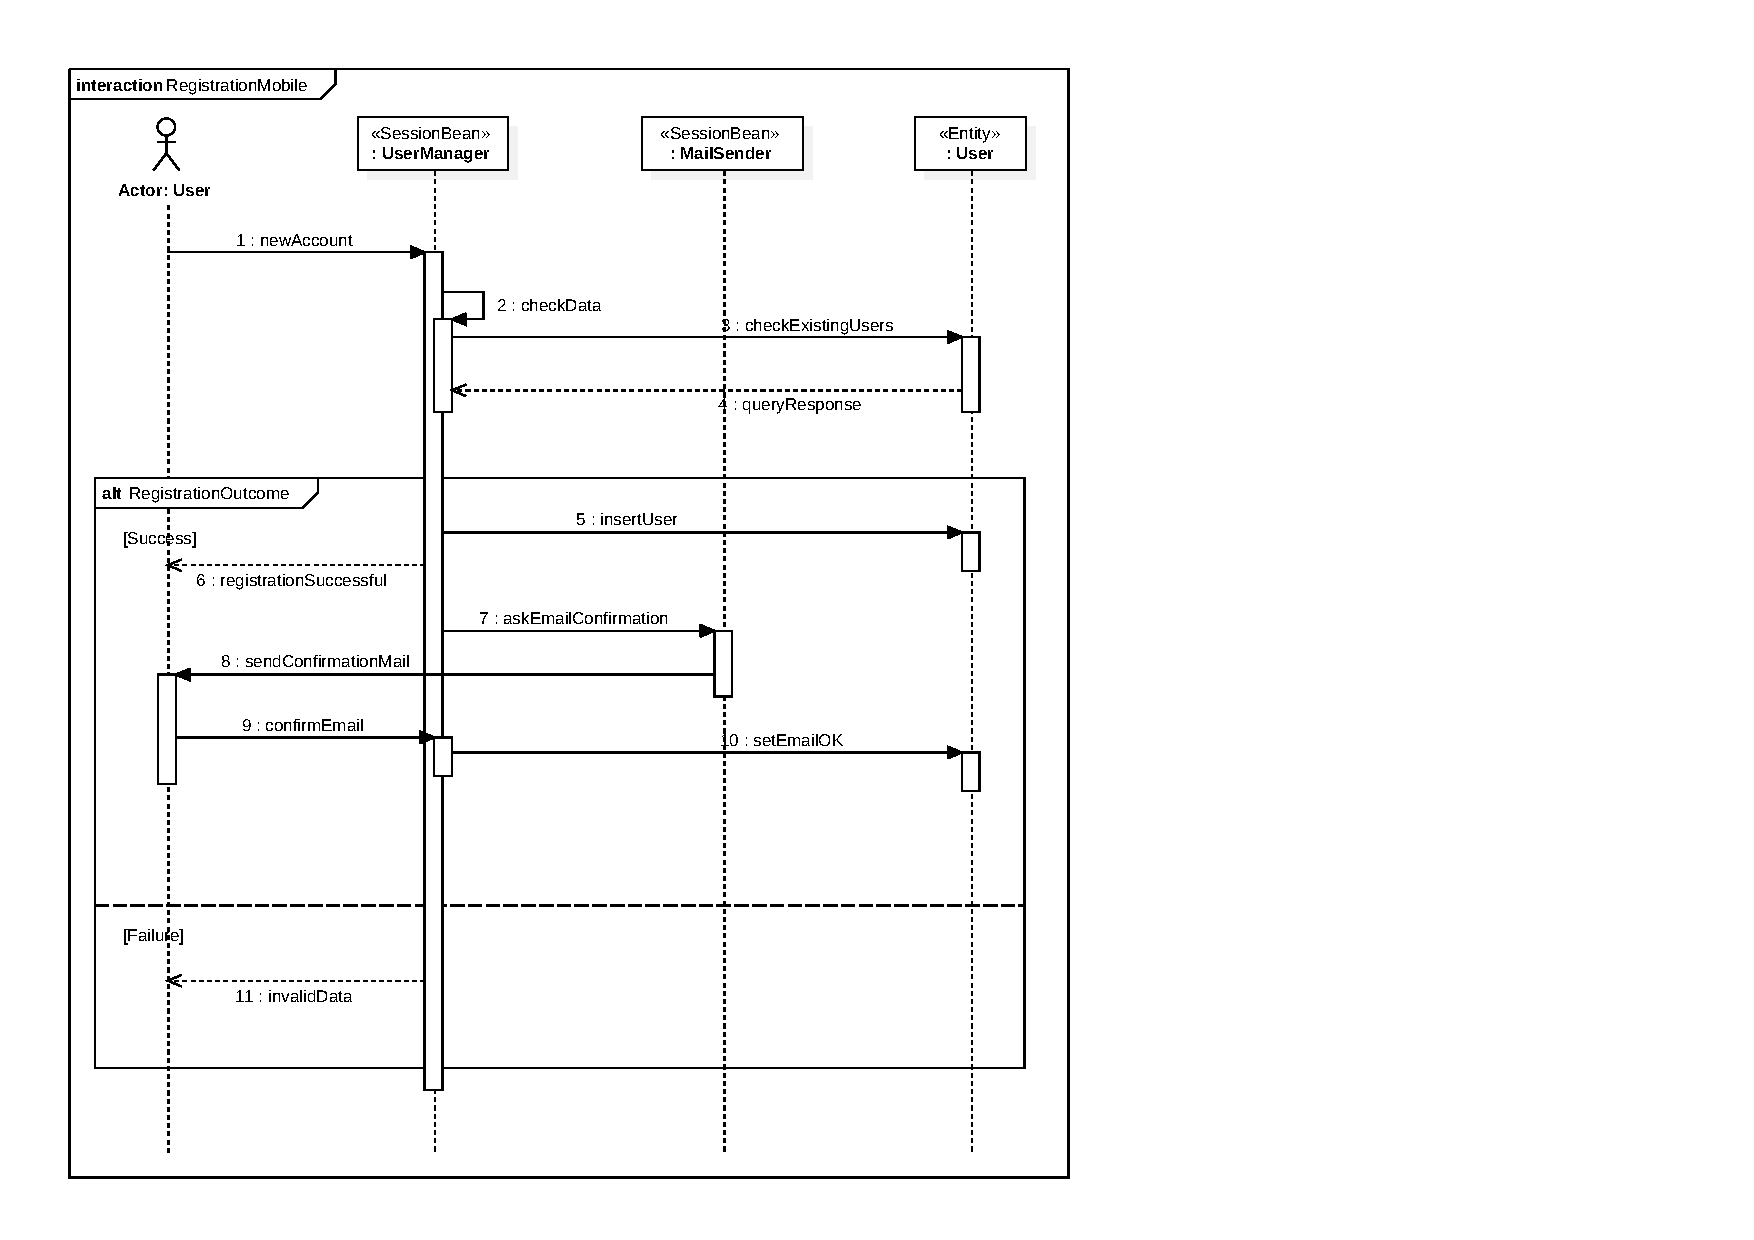
\includegraphics[width=\textwidth]{diagrams/sequence_registrationmobile}
    \caption{Sequence diagram of the registration from a mobile client.}
    \label{fig:sequence-registrationmobile}
\end{figure}

\begin{figure}[h]
    \centering
    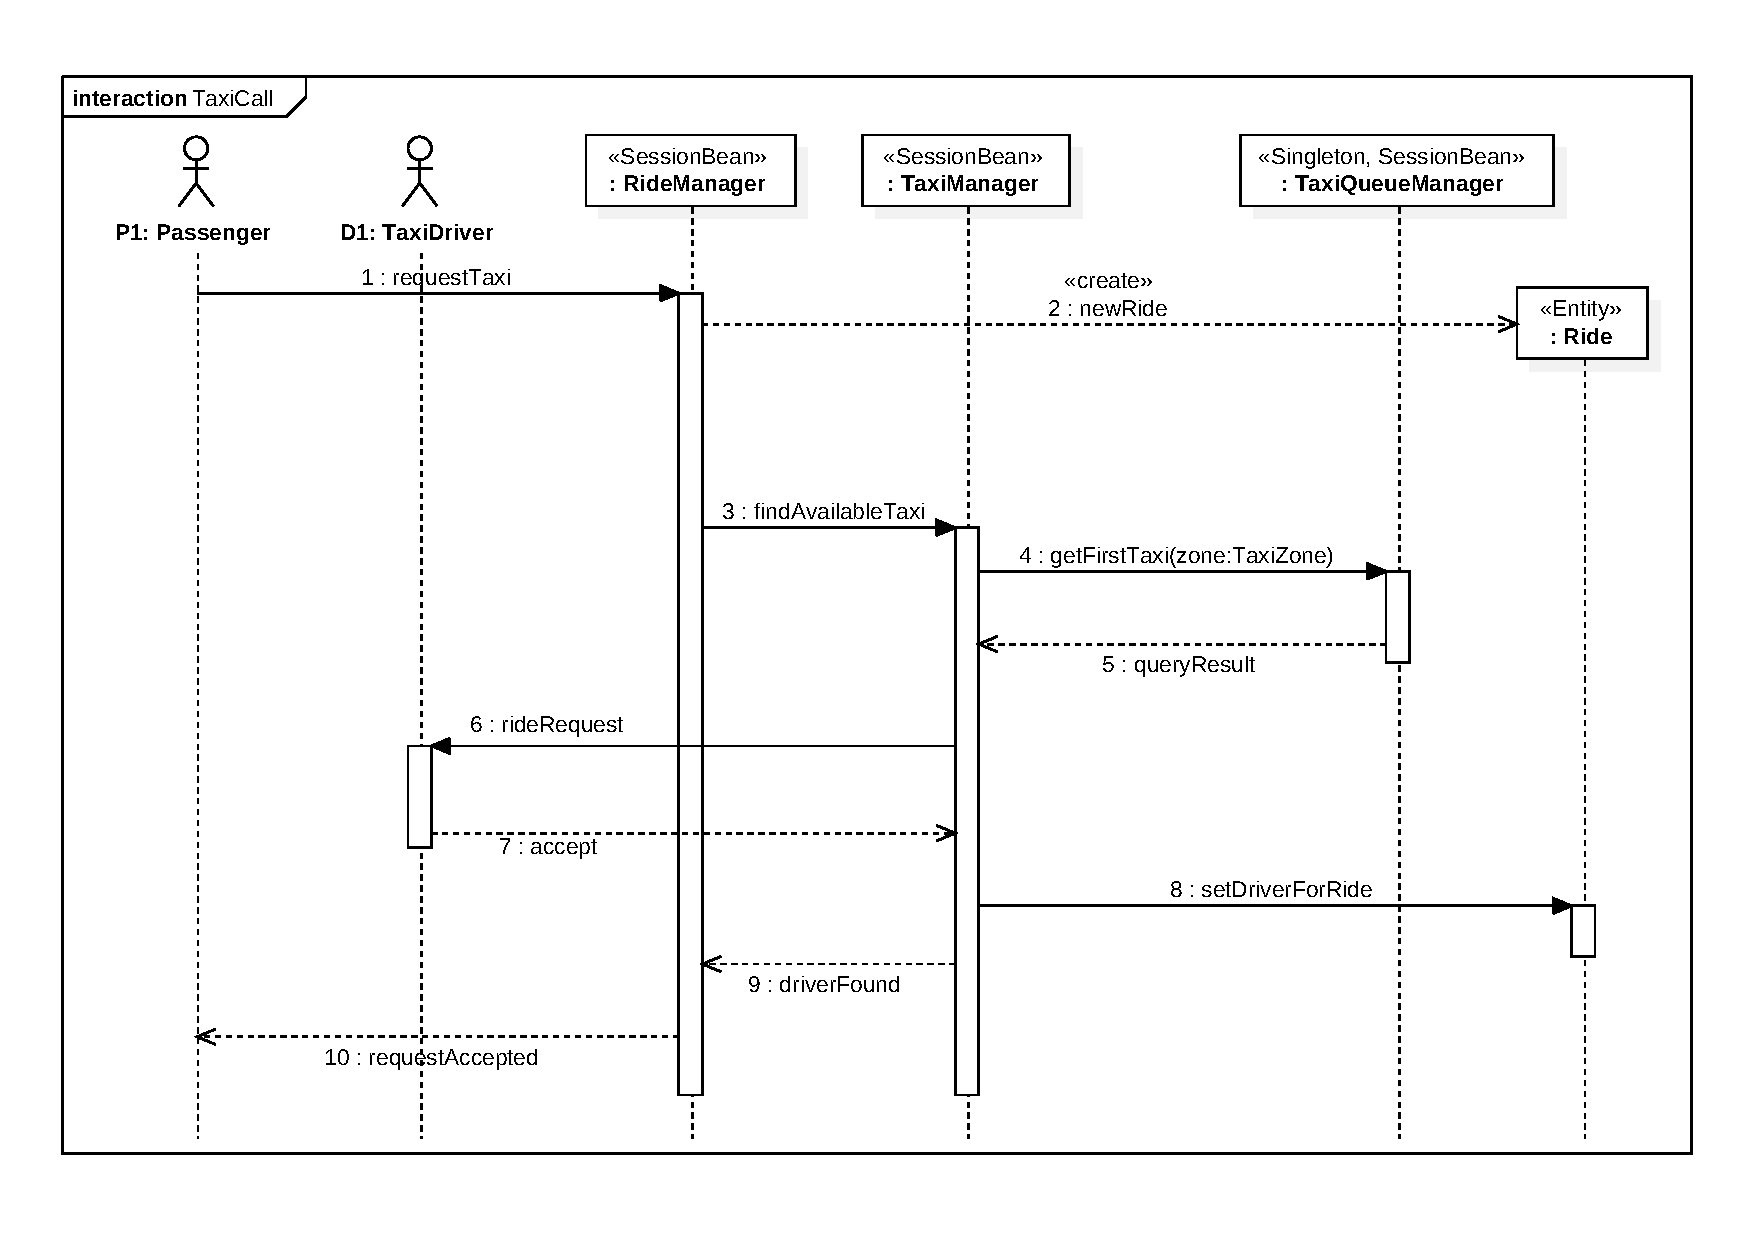
\includegraphics[width=0.85\textwidth]{diagrams/sequence_taxicall}
    \caption{Sequence diagram of a taxi call.}
    \label{fig:sequence-taxicall}
\end{figure}

\begin{figure}[h]
    \centering
    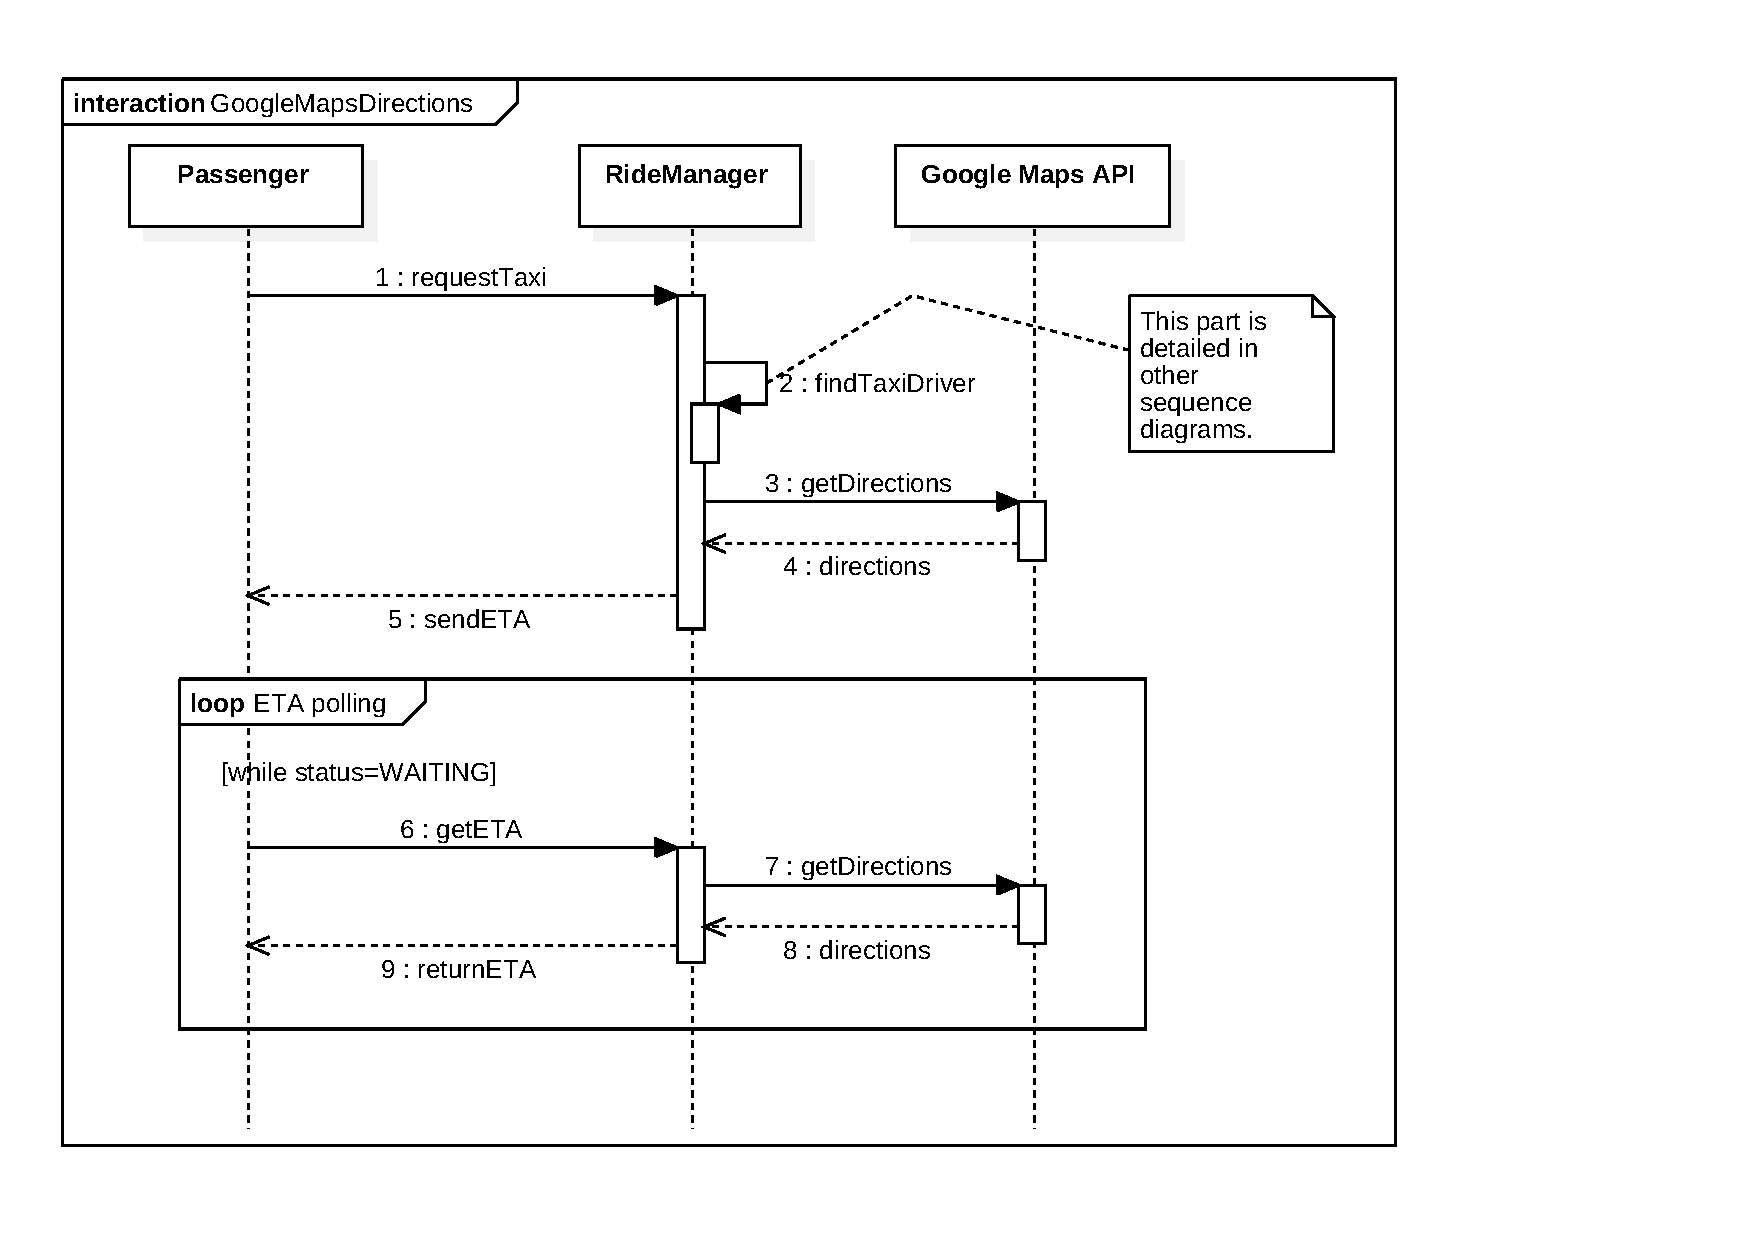
\includegraphics[width=0.85\textwidth]{diagrams/sequence_gmaps}
    \caption{Sequence diagram of the waiting time serivce, that uses the Google Maps Directions API detailed in~\autoref{sec:taxiwaiting}.}
    \label{fig:sequence-gmaps}
\end{figure}

\begin{figure}[h]
    \centering
    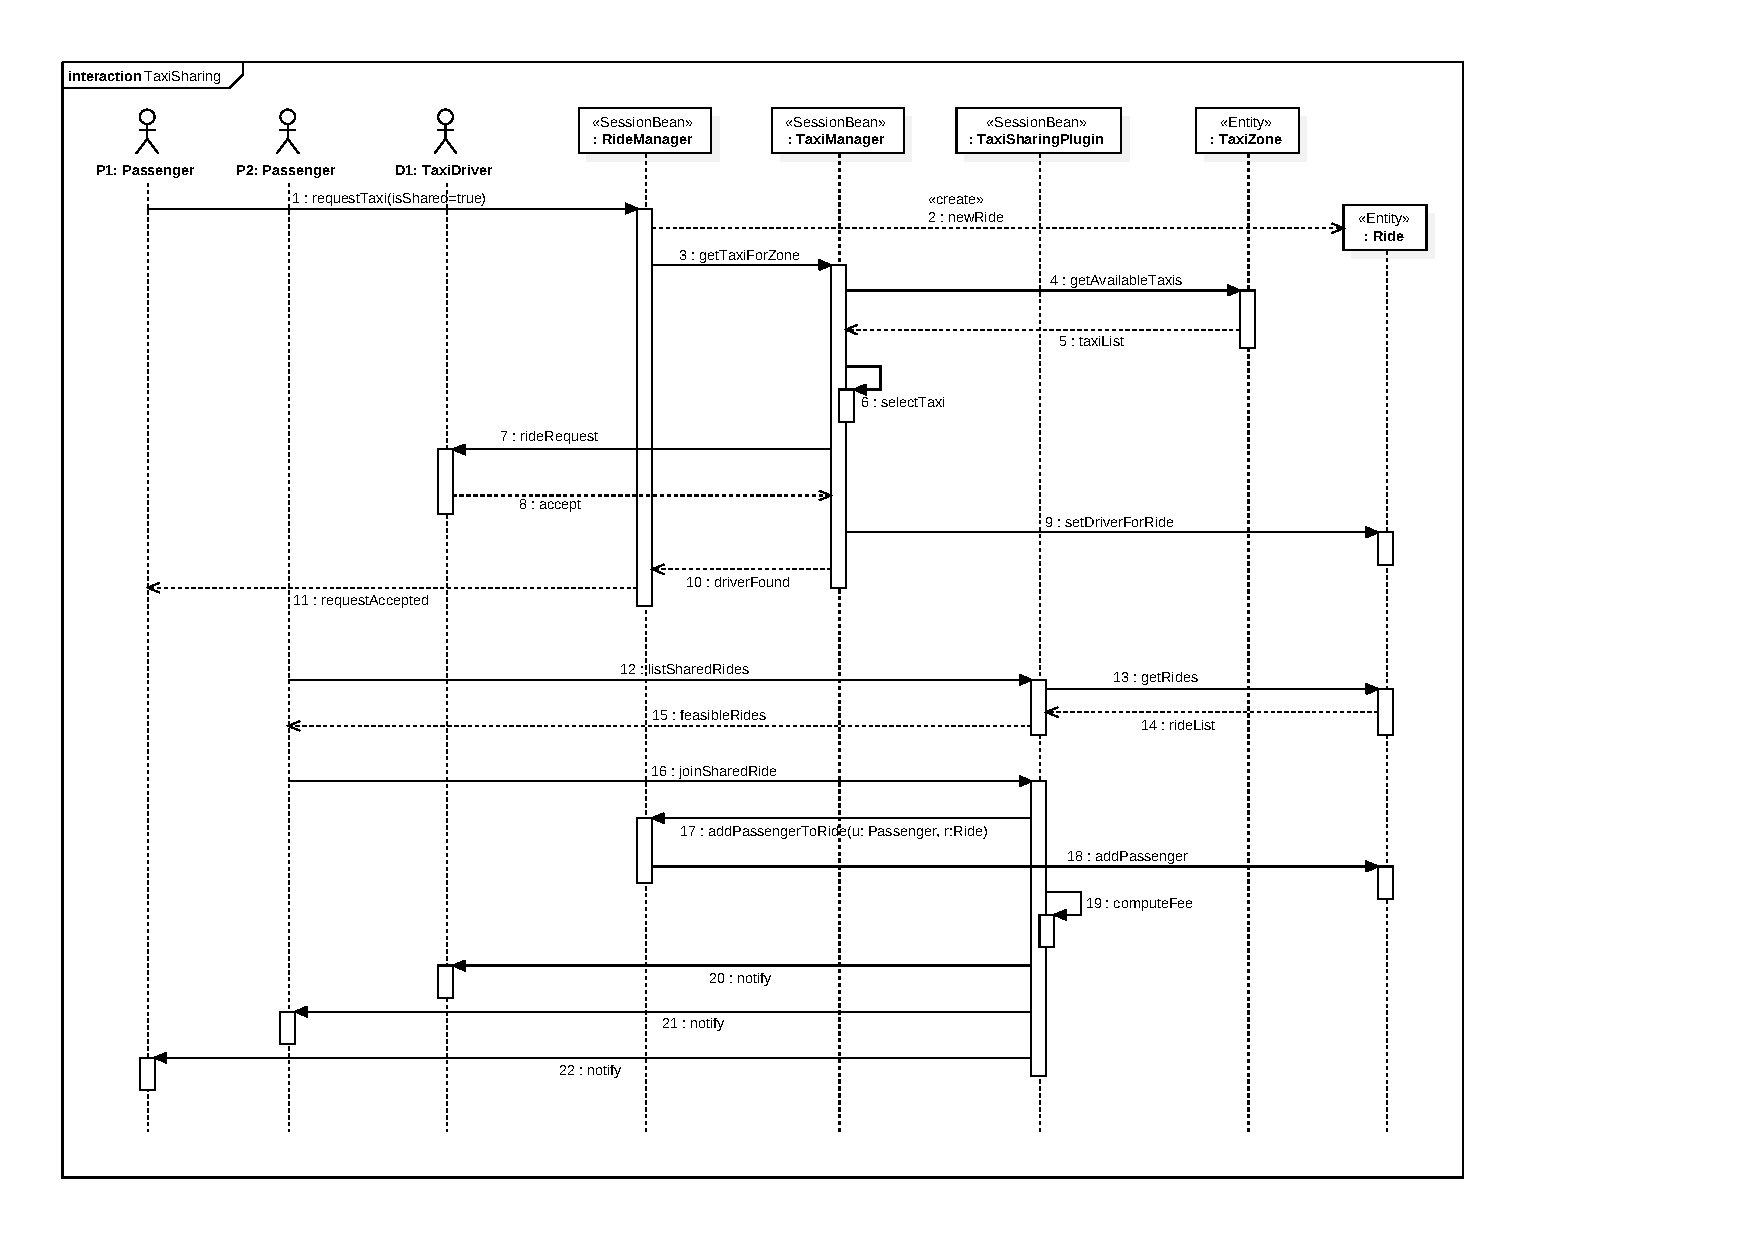
\includegraphics[width=\textwidth]{diagrams/sequence_taxisharing}
    \caption{Sequence diagram of a shared ride (2 passengers).}
    \label{fig:sequence-sharing}
\end{figure}

\FloatBarrier
